
\section{Periodiciteit en knoopfamilies}

Uit het bovenstaande emergeert een interessante parallel met het periodiek systeem. In de atoomtheorie wordt periodiciteit gedreven door elektronenschillen; in VAM lijkt een analoog principe op te duiken: knoopfamilies met vast $p$ vertonen capaciteitsgrenzen, waarna $p$ toeneemt (extra streng) en een nieuwe familie start. Dit verklaart qualitatiever de groepen elementen:

\textbf{Eerste periode (H, He):} Hier heeft waterstof al een $p=2$ knoop (trefoil) nodig voor stabiliteit. Men zou kunnen zeggen dat $p=2$ overeenkomt met de eerste “schil” van vortexstructuren, die echter maar 2 elementen bevat. Dit is vergelijkbaar met de $1s$ orbitaal die 2 elektronen opneemt. In VAM-termen is wellicht $p=2$ de minimaal mogelijke knoopstreng, die hooguit $q=3$ (H) en $q=5$ (He) toestaat als stabiele vormen. He heeft daarmee die $p=2$ capaciteit uitgeput (verder verhogen van $q$ leidt tot instabiliteit, wat we inderdaad bij Be zagen).

\textbf{Tweede periode (Li–Ne):} Deze corresponderen waarschijnlijk met knopen uit de $p=3$ familie (driestrengs knopen). Een $p=3$ knoop kan meer heliciteit opslaan zonder instabiliteit dan een $p=2$. Mogelijk begint Li (Z=3) al als $p=2$ ($T(2,7)$ in onze tabel), maar het zou ook kunnen dat vanaf Beryllium of Boor de omslag naar $p=3$ gebeurt. Indien Li t/m Ne door $p=3$ knopen worden gedragen, zou die familie tot 8 elementen kunnen omvatten, vergelijkbaar met de 2e elektronenschil. Het onderscheid tussen $p=2$ en $p=3$ knopen zou subtiel kunnen inzetten rond beryllium/boor, wat misschien het bestaan van de instabiele $^8$Be verklaart: $^8$Be zou precies op de overgang liggen – als twee gekoppelde $p=2$ knopen (twee alpha’s) stabieler zijn dan één slecht passende $p=3$ knoop, valt $^8$Be uiteen. Zodra we bij boor/koolstof zijn, domineert $p=3$ waarschijnlijk, en die reeks kan doorlopen t/m Ne.

\textbf{Derde en vierde periode:} Deze bevatten 8 resp. 18 elementen. In VAM zouden dit $p=4$ en $p=5$ knoopfamilies kunnen zijn. Een $p=4$ (vierstrengs) torusknoop heeft potentieel ruimte voor meer complexe linking (mogelijk tot 18 stabiele configuraties) voordat een $p=5$ nodig is. IJzer-groep (periode 4 midden) zou dus $p=4$ knopen zijn, wat hun hoge stabiliteit ondersteunt. Daarna, vanaf rubidium (Z=37), zou $p=5$ starten, samenhangend met de 18 elementen in periode 5.

% --- Figuur 4: Periodieke knoopfamilies ---
\begin{figure}[H]
    \centering
    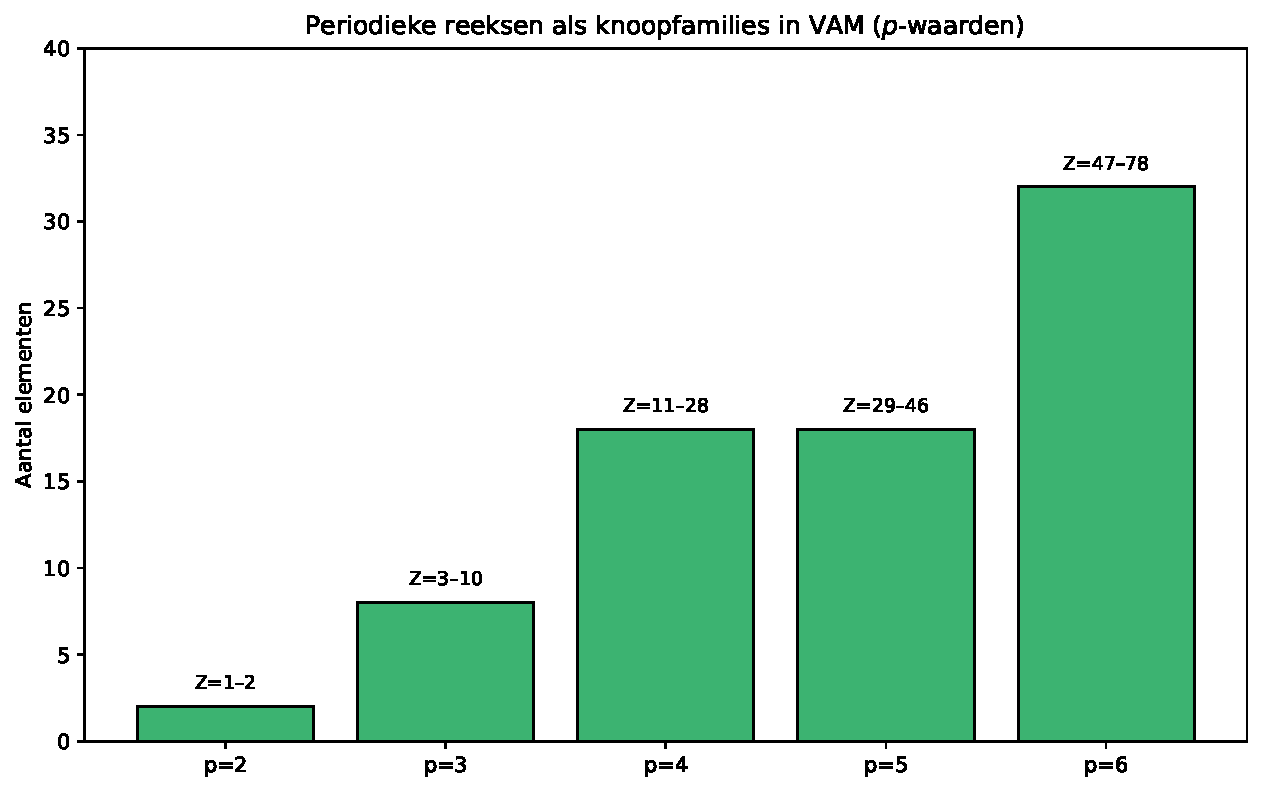
\includegraphics[width=0.65\textwidth]{sections/4_KnoopFamilies}
    \caption{Aantal elementen per knoopfamilie $p$, overeenkomend met periodieke reeksen in het klassieke systeem.}
    \label{fig:knoopfamilies}
\end{figure}

\textbf{Vijfde en zesde periode:} Periode 6 heeft 32 elementen, wat in dit patroon $p=6$ familie zou zijn. Inderdaad worden de langste perioden gedragen door zeer complexe knopen (6- of 7-strengs). Deze kunnen zeer veel $q$ variatie aan tot ze vol raken. Uiteindelijk bij superzware elementen (boven uranium) zou zelfs $p=7$ niet meer afdoende zijn en treedt op wat we al beschreven: multi-knoop samenstellingen in plaats van één knoop.

Deze topologische periodiciteit is momenteel een kwalitatieve analogie, maar het is opmerkelijk hoe de getallen ruwweg overeenkomen met $2, 8, 18, 32$ elementen per knoopsoort. Het suggereert dat natuurwetten op fundamenteel niveau misschien een weerspiegeling zijn van topologische combinatoriek: net zoals elektronen permutaties van quantumtoestanden volgen, volgen protonen in VAM permutaties van streng- en winding-combinaties.

Periodieke trends in chemische eigenschappen (valentie) zouden in VAM vertaald moeten worden naar bepaalde symmetrische eigenschappen van knopen. Bijvoorbeeld, edelgassen (He, Ne, Ar, Kr, Xe) corresponderen met volledig gevulde knopenfamilies – wellicht knopen waarbij $q$ een maximale stabiele waarde heeft bereikt voor gegeven $p$, waardoor de vortexstructuur “gesloten” is en geen reactiviteit (valentie) vertoont. Omgekeerd zouden alkali-metalen (H, Li, Na, K, Cs, Fr) telkens het begin van een nieuwe knoopfamilie zijn: één winding in een nieuwe strengconfiguratie bovenop een voltooide vorige – in VAM-termen misschien knopen waarin één streng dominant $q$ heeft en de rest nauwelijks bijdraagt, resulterend in een unpaired heliciteit kwantum dat makkelijk interactie aangaat (valentie 1).

Dit soort analogieën zijn speculatief, maar het VAM-raamwerk is rijk genoeg om dit soort systematiek voort te brengen: topologische restricties kunnen leiden tot families van structuren met vergelijkbare gedragingen, net zoals quantumrestricties dat doen in het traditionele atoommodel. Een belangrijk verschil is dat VAM alles terugbrengt tot continuümmechanica: de “shells” zijn geen abstracte orbitaalwolken maar concrete vortexconfiguraties.
